%%This is a very basic article template.
%%There is just one section and two subsections.
%\documentclass[12pt,oneside,a4paper,doublespacing]{article} % for submission
\documentclass[12pt,oneside,letter]{article} % for sharing

\usepackage{appendix}
\usepackage{amsmath}
\usepackage{caption}
\usepackage{placeins}
\usepackage{graphicx}
\usepackage{subcaption}
%\usepackage{subfig}
\usepackage{longtable}
\usepackage{setspace}
%\usepackage{tikz}
\usepackage{booktabs}
\usepackage{tabularx}
\usepackage{xcolor,colortbl}
\usepackage{chngpage}
%\usepackage[active,tightpage]{preview}
\usepackage{natbib}
\bibpunct{(}{)}{,}{a}{}{;} 
\usepackage{url}
\usepackage{nth}
\usepackage{authblk}
\usepackage[most]{tcolorbox}
%\usepackage{hyperref}
%\usepackage{color}
%\usepackage{fontspec}
%\usepackage{pdfsync}
\usepackage[normalem]{ulem}
\usepackage{amsfonts}
\renewcommand{\listtablename}{List of Appendix Tables}
\newcolumntype{C}[1]{>{\centering\let\newline\\\arraybackslash\hspace{0pt}}m{#1}}
\newcolumntype{L}[1]{>{\raggedright\let\newline\\\arraybackslash\hspace{0pt}}m{#1}}
% working on this need to concatenate file name based on sex and variable name
%\newcommand\Cell[1]{{\raisebox{-0.05in}{\includegraphics[height=.2in,width=.2in]{Figures/ColorCodes/\expandafter#1}}}}  

%%%%%%%%%%%%%%%%%%%%%%%%%%%%%%%%%%%%%%%%%%%%%%%%%%%%%%%%%%%%%%%%%%%%%%%%%%%%%
% setting color to letters affects spacing. Here's a hack I found here:
% http://tex.stackexchange.com/questions/212736/change-letter-colour-without-losing-letter-spacing
%\DeclareRobustCommand{\spacedallcaps}[1]{\MakeUppercase{\textsc{#1}}} % all
% caps with better spacing

%\colorlet{RED}{red}
%\colorlet{BLUE}{b}
\colorlet{rd}{red}
\colorlet{bl}{blue}

%%%%%%%%%%%%%%%%%%%%%%%%%%%%%%%%%%%%%%%%%%%%%%%%%%%%%%%%%%%%%%%%%%%%%%%%%%%%%%

\newcommand\ackn[1]{%
  \begingroup
  \renewcommand\thefootnote{}\footnote{#1}%
  \addtocounter{footnote}{-1}%
  \endgroup
}
\newcommand\vt[1]{\textcolor{rd}{#1}}
\newcommand\eg[1]{\textcolor{bl}{#1}}

\newcommand\tg[1]{\includegraphics[scale=.5]{Figures/triadtable/triad#1.pdf}}
\newcommand\tgh[1]{\raisebox{-.25\height}{\includegraphics[scale=.3]{Figures/triadtable/triad#1.pdf}}}

\defcitealias{HMD}{HMD}

% junk for longtable caption
\AtBeginEnvironment{longtable}{\linespread{1}\selectfont}
\setlength{\LTcapwidth}{\linewidth}

%%%%%%%%%%%%%%%%%%%%%%%%%%%%%%%
\begin{document}

\title{A unified framework of demographic time}

\author[1]{Tim Riffe\thanks{triffe@demog.berkeley.edu}}
\author[2,3]{Jonas Sch{\"o}ley}
\author[2,3]{Francisco Villavicencio}
\affil[1]{Max Planck Institute for Demographic Research}
\affil[2]{University of Southern Denmark}
\affil[3]{Max-Planck Odense Center on the Biodemography of Aging}

%\author{[Authors]}

\maketitle

\begin{abstract}
We describe a three-dimensional relationship between six different measures
of demographic time. The six measures of demographic time considered are
chronological age, time to death, lifespan, time of birth, time of
death, and period. We describe four identities among subsets of these six
measures, and then a full identity that relates the six of them. \ackn{The work reported in this manuscript was begun by
the first author while at the Department of Demography at the University of
California, Berkeley, and was supported by the U.S.
National Institute On Aging of the National Institutes of Health under award
numbers R01-AG011552 and R01-AG040245. The content is solely the responsibility of the authors and does not necessarily represent the official views of the funding agencies.}
\end{abstract}

\section*{Introduction}
%\sout{so-called} \textbf{well-known?} 
In the course of training, all demographers are introduced
to the Lexis diagram, a convenient graphical identity between the three main
time measures used to structure demographic stocks and flows: Age, period, and birth cohort.
This popular representation does not account for remaining years of life and
other related time indices that may be of great interest to researchers and
policy makers. % The Lexis diagram relates the chronological age (A), period (P),
% and birth cohort (C) measures of demographic time, APC, but it does not account
% for remaining years of life (thanatological age), and other related time
% indices.
We identify three time indices that are complementary to age (A), period (P) and
birth cohort (C). The first such index is time-to-death, which we refer to as ``thanatological age'' (T) in contrast to ``chronolgocial age'' (A). The second index is death cohort (D), which groups
all individuals (of different ages) dying in the same time period. Finally,
lifespan (L) is itself an index by which data may be structured. We therefore
have six time measures in total to relate.

Just as the Lexis diagram has been a fundamental instrument to
teach demography for decades, we hope that the demographic time measures and
their graphical depictions presented here will be helpful to teachers and
young demographers. The temporal relationships we describe will also be useful
for researchers to better understand the temporal structure of data, and for methodologists to
better account for the temporal structure of data in demographic methods.
We believe in the pedagogical value of the concepts and tools introduced in the
following pages. 

The Lexis diagram can be understood as an APC plane
that relates age (A), period (P), and birth cohort (C). Other such planes also
exist. The ``thanatological'' counterpart to APC is an identity between
thanatological age (T), period (P), and death cohort (D), TPD. A third identity
relates thanatological age (T), chronological age (A), and lifespan (L), TAL. Finally, a potentially less
intuitive graphical identity relates lifespan (L), birth cohort (C), and death
cohort (D), LCD. We call three-way identities of this sort ``triad identities''.
% The thanatological counterpart to APC is an identity between thanatological
% age (T), period (P), and death cohort (D), TPD. A third
% identity exists between thanatological age (T), chronological age (A), and
% lifespan (L), TAL, and a fourth between lifespan (L), year of birth (C) and year
% of death (D), LCD.

Each of these four triad identities (APC, TPD, TAL, and LCD) may be sufficiently described by any two of its constituent indices, making the third index redundant. For instance, if the age (A) of an individual in a particular time period (P) is known, the birth cohort (C) to which he or she belongs can be immediately derived. Moreover, each of these four identities also lacks a major dimension of time. The TAL identity lacks calendar time, the LCD identity is ageless, APC lacks an endpoint in time, and TPD lacks a starting point in time.
% Each of these four identities may be sufficiently described by any
% two of its consituent indices, making the third index redundant. Each of these
% four identities also lacks a major dimension of time. The TAL identity
% lacks calendar time, the LCD identity is ageless, APC lacks an endpoint in time,
% and TPD lacks a starting point in time. We refer to these four identities
% as the triad identities.
To our knowledge, the only triad identity that has received serious
treatment at the time of this writing is the APC identity. Different
aspects of the APC identity have been discussed since at least 1868
\citep{knapp1868ermittlung}, and discussion remains lively today. Here we relate the six major indices of time in a geometric identity, in much the same spirit as the work on APC relationships done between the late
1860s and mid 1880s.\footnote{See e.g., \citet{keiding2011age} for an overview of that literature.} 

The objective of this paper is to describe the geometric identity between all
six measures of demographic time, a hexad identity, that may be useful or an intuitive
referent for demographers in the same way as the Lexis diagram. At the same time, this identity relates the
four triad identities we have mentioned. We give a bottom-up
description of how the six dimensions of time relate in a single framework,
building from familiar components to the full relationship.
We begin by defining some terms used throughout the manuscript. We then explore all combinations of two time
measures, the dyadic relationships, followed by the four triad identities, and
finally the hexad identity. We give a systematic topological overview of the
different elements of demographic time. 
%This paper contains no data visualizations, but it may serve as a basis for designing some.

\section*{Definitions}
\subsection*{Technical terminology}
We attempt to adhere to a rigorous terminology in this paper. The following list
describes some of the more important terms we use.
\begin{description}
\item[Time measures] are any of the six time indices discussed to describe demographic time: chronological age (A), period (P), birth cohort (C), thanatological
age (T)\footnote{Elsewhere in the literature, thanatological age is known
as residual life, time-to-death, remaining years, or simply years left.}, lifespan (L), and death
cohort (D).
\item[Dyads, triads, and hexads] are any set of two, three, or six unique time
measures, respectively.
\item[An informative dyad] is any pair of two time measures from which a third
time measure can be derived. For example, A and P form an informative dyad from which C can be derived.
%\item\sout{[Given measures] are any specified set of time measures.}
%\item\sout{[Derived measures] are any unspecified time measures that are implied by or
%derived from a given set.} 
%\item\sout{[An informative] set is a set of given measures that entails at
%least one derived measure.}
%\item\sout{[An uniformative] set is a set of given measures that does not entail any
%derived measures.}
\item[A triad identity] is the union of an informative dyad and
its one derived time measure. Analogously, a triad identity is the union of
three different time measures, with the property that any of them can be derived from the other two with no additional information. There are four triad identities: APC, TPD, TAL and CDL.
%\item[A hexad identity] is a unique combination of the six time measures.
\item[A temporal plane] is any $(x,y)$-mapping of a dyad of time measures.
\item[A temporal space] is any $(x,y,z)$-mapping of a triad of time measures.
\end{description}
Using this terminology, we say that the ``Lexis'' measures
constitute a triad identity between chronological age, period, and birth cohort. Each dyad
combination of elements in this identity is informative, and can be mapped to a
temporal plane, the Lexis diagram. If we know that Mindel turned 50 on the
\nth{21} of May, 1963, then we also also can derive that she was born on the \nth{21} of
May, 1913. Any two pieces of information in this case will give the third, which
means that any dyad from this set is informative. Three other such triad
identities are also to found within the six measures of time we discuss.
However, as we describe in later sections, not all sets of three time measures
yield the full set of six, the hexad identity. Thus, some triads are
informative, and others are uniformative. It turns out that each of the triad identities is uninformative in
this sense.

\FloatBarrier

\subsection*{Time measures}
\FloatBarrier
Our model description is conceived in absolute, linear, Newtonian time, and we
do not consider situating the model in any other perspective on or notion of
time itself.
This relationship is scalable to any time unit, but we decribe it in terms of
years, the dominant time scale for human demography. We therefore speak of
calendar time, imagining the modern Gregorian calendar, though this is not
necessary. We also describe the model in terms of human lifespans, although it
applies in a more general sense to any durations observed over time.
The six measures of time we consider are defined in Table~\ref{tab:sixdefs}, both in the demographic sense we describe, as well as in a more general event history interpretation.

%\begin{adjustwidth}{-3em}{-3em}

\begin{table}
\centering
\caption{Definitions of the six time measures.}
\label{tab:sixdefs}
\begin{adjustwidth}{-2em}{-2em}
\begin{tabular}{lcll}
\hline 
\textbf{Time measure} & \textbf{Short} & \textbf{Demographic def.} &
\textbf{Event history def.}\\
\hline 
chronological age & A & Time since birth & Time since start of exposure \\
period & P & calendar time & calendar time \\
birth cohort & C & calendar time of birth & calendar time of exposure start \\
thanatological age & T & time until death & time until event \\
death cohort & D & calendar time of death & calendar time of event \\
lifespan & L & duration of life & duration of exposure \\
\end{tabular}
\end{adjustwidth}
\end{table}

Each of the time measures except for period are governed by the processes of
birth and/or death. For this reason we call this a model a demographic time.
The concepts of thanatological age and death cohorts are likely less familar to
readers than the other measures we consider. Thanatological age is sometimes
referred to in the literature as remaining years of life, time-to-death (TTD),
or residual lifespan, but we prefer the term thanatological age. Age in this
general sense marks a position on a lifeline with respect to one of its
endpoints.
Chronological age and thanatological age are in this way
complementary.\footnote{Thanatological age is different from the notion of
prospective age, used by \citet{sanderson2007new}, since prospective age is a relative term that reflects
a comparison of expectancies. Prospective age scales chronological age by
comparing mortality schedules, but it is neither an expectancy nor a statement
of remaining years of life.} Thanatological age is meaningful without much
justification; it is the measure we all want to know, the thing we approximate
with remaining life expectancy.

Cohorts in general associate individuals that share a characteristic. In
demography the grouping characteristic is often a combination of place and time, such as
the cohorts of young demographers passing through a particular graduate program.
In this instance already, we accomodate the notion of a cohort for both the
start and endpoints of the program, but we say e.g., ``the class of 2015''
instead of the ``graduating cohort of 2015'', in contrast to ``cohort 37'', the
\nth{37} class of entering students since the start of the program.
These concepts are analagous to the ideas of birth and death cohorts we use
here, but we do not often refer to the deaths of a given year as a death cohort.
In the time preceding death, the members of a given death cohort have much in common, despite
heterogeneity with respect to time of birth.\footnote{Death cohorts lack a
shared identity, so any kind of emergent homogeneity in a death cohort probably
has a physiological basis.} If the reader accepts this premise, then the
abstract construct of a death cohort is also meaningful in the way that other cohort measures are.

Much of the work of demography is directed at the study of lifespan. Lifespan is
synonymous both with longevity, chronological age at death, and thanatological
age at birth. One's ultimate completed lifespan is constant throughout life,
though we have no knowledge of it until death: It is assigned retrospectively.
Demographers have more often used lifespan or age-at-death as a measure of mortality, or similar, than as a measure on which to compare individuals. 

Treating lifespan,
death cohorts, and thanatological age as temporal structuring variables
enables new classes of comparisons, models of understanding, and discovery,
akin to those unlocked by breaking down demographic phenomena by chronological age,
period, and birth cohort. The following sections will, in this sense, provide an
exhaustive classification of the ways in which these six measures of time can be juxtaposed to such ends.
We begin with all sets of two time measures, the informative and uninformative
temporal dyads.

\FloatBarrier

\section*{Informative and uninformative dyads}

Any mapping of two time measures to an ($x,y$) coordinate
system constitutes a temporal plane. If the two given time measures are members of the same triad identity, the third member is called a derived
measure. For instance, if we take the dyad $AP$, $C$ is the derived
measure, making $AP$ an informative dyad. We make this dyadic relationship
explicit by writing $AP(C)$.
The temporal plane that corresponds to this informative dyad is the contemporary representation of the
Lexis diagram. The informative dyads $AC(P)$ and $CP(A)$ also belong to the Lexis identity, but imply different less-common rotations and projections of the Lexis
diagram. 

For each dyad there is a fundamental question of how to map the constituent
coordinates to a cartesian temporal plane. Typically one forces parity between time units within
a specified dyad, and maps one element directly to $x$ and the second element
directly to $y$, resulting in a 90$^\circ$ angle between the $x$ axis and $y$
axis. In this case the convention is to force a unity aspect ratio
between the $x$ and $y$ axes, such that the derived measure, if any, is then
\textit{accidentally} present in a 45$^\circ$ ascending or descending angle,
depending on the dyad and axis orientation. 

It has long been noted \citep{zeuner1869abhandlungen, perozzo1880della} that the
derived time measure, when plotted at 45$^\circ$, is relatively
longer than either the age or period axes. If a right angle and unity aspect
ratio is forced between the dyad, the derived measure is always stretched by
$\sqrt{2}$, or 41\%. In the case of dyads that imply a derived measure, another
logical mapping is to translate to $(x,y)$ coordinates that forces 60$^\circ$
angles between the three measures. Such a mapping ensures that the spatial units are equal for the three measures, and we therefore refer to it as the isotropic mapping. It does not make sense to provide an isotropic mapping of an uninformative dyad. The isotropic mapping
is comparable to using ternary or baricentric coordinate systems, which we do
not discuss. 
%The primary justification for isotropic temporal planes comes from
%a data visualization perspective, where it may be hypothesized that the
% viewer's ability to compare slopes is hindered if the axes are not on the same scale.
Under the isotropic mapping, the three variants of each triad identity are
simple rotations of one another, and they imply no rescaling.

There are $15=\binom{6}{2}$ possible ways to form a dyad from our set of six time measures, 12 of
which are informative, and three of which have no derived time measure, and are
therefore called uninformative. These dyads, an explanation or simple example,
and the corresponding graphical representations are summarized in
Table~\ref{tab:dyads}. Each informative dyad is a subset consisting of two
elements from one of the four triad identities (APC, TPD, TAL, LCD), which we
analyze in detail in further sections. The uninformative dyads are simply a pairs of time measures that are not contained in any of these four
triad identities.

\begin{longtable}{m{0.13\textwidth}m{0.37\textwidth}m{0.17\textwidth}m{0.17\textwidth}}
  \caption{All dyadic juxtapositions of the six measures of demographic time.}
  \label{tab:dyads}\\
 
  \toprule
  \multicolumn{4}{m{0.9\textwidth}}{\footnotesize \emph{Note:} The temporal planes are named after the two given time scales. The derived scale is appended in parentheses. Contrary to mathematical convention we name the ordinate scale first and the abscissa scale second. This is to be consistent with the established $APC$ and $ACP$ terms.} \\
  \midrule
  \multicolumn{1}{c}{relationship} & \multicolumn{1}{c}{description} &
  \multicolumn{1}{c}{Cartesian} & \multicolumn{1}{c}{isotropic} \\
  \midrule
  %%%%%%%%%%%%%%%%%%%%%%%%%%%%%%%%%%%%%%%%%%%%%%%%%%%%%%%%%%%%%%%%%%%%%%%%%%%%%
  \multicolumn{4}{c}{\textsc{Variants of APC}} \\
  \midrule
  %%%% APc
  $$\begin{aligned}
    &AP(C) \\
    &C = P - A
  \end{aligned}$$ &
  The $AP(C)$ temporal plane constitutes the classical Lexis diagram. &
  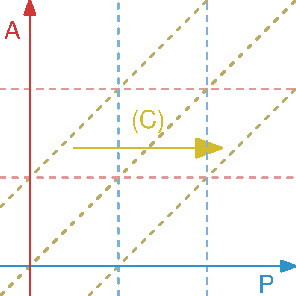
\includegraphics[height = 2cm]{Figures/JonasTable/APc-crop.pdf} &
  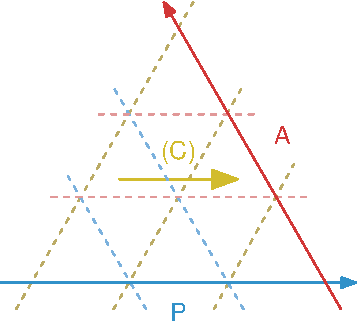
\includegraphics[height = 2cm]{Figures/JonasTable/APc_iso-crop.pdf}  \\
  %%%% ACp
  $$\begin{aligned}
    &AC(P) \\
    &P = C + A
  \end{aligned}$$ &
  The $AC(P)$ temporal plane is equivalent to the Lexis diagram only that birth cohort is given and period is embedded instead of the other way round. &
  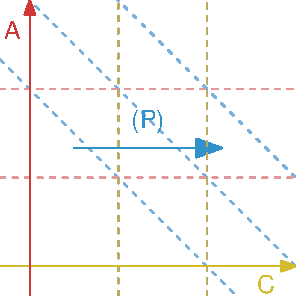
\includegraphics[height = 2cm]{Figures/JonasTable/ACp-crop.pdf} &
  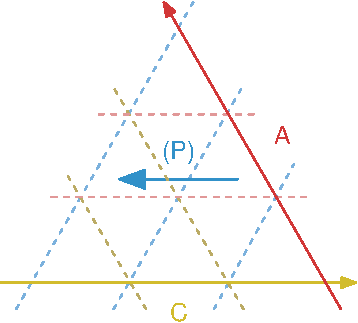
\includegraphics[height = 2cm]{Figures/JonasTable/ACp_iso-crop.pdf}  \\
  %%%% CPa
  $$\begin{aligned}
    &CP(A) \\
    &A = P - C
  \end{aligned}$$ &
  The $CP(A)$ temporal plane is equivalent to the Lexis diagram only that birth cohort is given and age is embedded instead of the other way round. &
  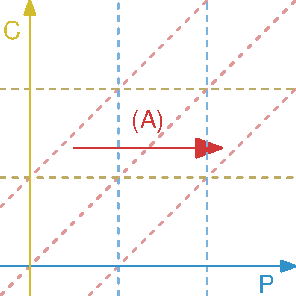
\includegraphics[height = 2cm]{Figures/JonasTable/CPa-crop.pdf} &
  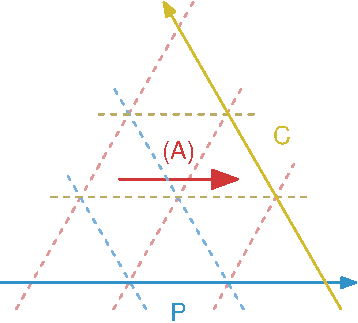
\includegraphics[height = 2cm]{Figures/JonasTable/CPa_iso-crop.pdf}  \\
  \midrule
  %%%%%%%%%%%%%%%%%%%%%%%%%%%%%%%%%%%%%%%%%%%%%%%%%%%%%%%%%%%%%%%%%%%%%%%%%%%%%
  \multicolumn{4}{c}{\textsc{Variants of TPD}} \\
  \midrule
  %%%% TPd
  $$\begin{aligned}
    &TP(D) \\
    &D = P + T
  \end{aligned}$$ &
  Helen had 30 years of life left ($T$) in 1971 ($P$) and therefore belonged to the 2001 death cohort ($D$) &
  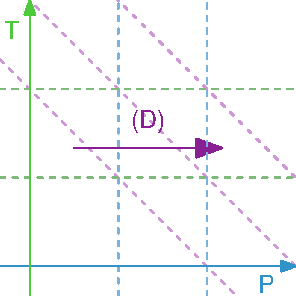
\includegraphics[height = 2cm]{Figures/JonasTable/TPd-crop.pdf} &
  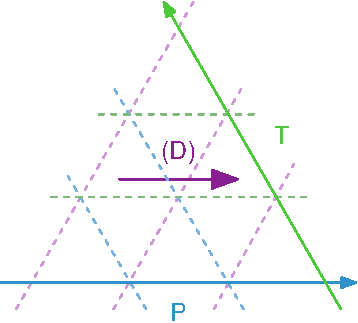
\includegraphics[height = 2cm]{Figures/JonasTable/TPd_iso-crop.pdf}  \\
  %%%% PDt
  $$\begin{aligned}
    &PD(T) \\
    &T = D - P
  \end{aligned}$$ &
  Mindel died in 1973 ($D$). In 1953 ($P$) she had 20 years left to live ($T$). &
  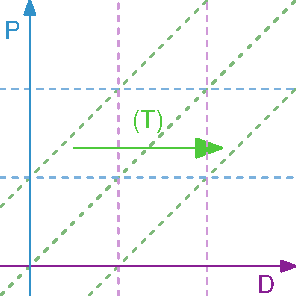
\includegraphics[height = 2cm]{Figures/JonasTable/PDt-crop.pdf} &
  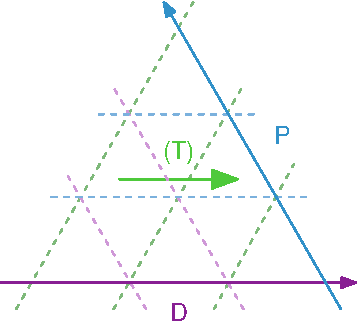
\includegraphics[height = 2cm]{Figures/JonasTable/PDt_iso-crop.pdf}  \\
  %%%% TDp
  $$\begin{aligned}
    &TD(P) \\
    &P = D - T
  \end{aligned}$$ &
  Irene died in 1974 ($D$). When she had 30 remaining years of life ($T$) the year must have been 1944 ($P$). &
  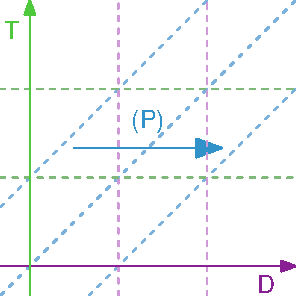
\includegraphics[height = 2cm]{Figures/JonasTable/TDp-crop.pdf} &
  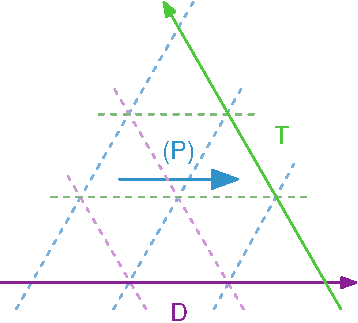
\includegraphics[height = 2cm]{Figures/JonasTable/TDp_iso-crop.pdf}  \\
  \midrule
  %%%%%%%%%%%%%%%%%%%%%%%%%%%%%%%%%%%%%%%%%%%%%%%%%%%%%%%%%%%%%%%%%%%%%%%%%%%%%
  \multicolumn{4}{c}{\textsc{Variants of TAL}} \\
  \midrule
  %%%% TAl
  $$\begin{aligned}
    &TA(L) \\
    &L = T + A
  \end{aligned}$$ &
  The time already lived and the time still left sum up to the total lifespan. &
  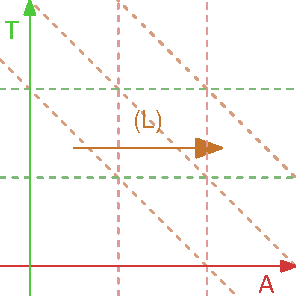
\includegraphics[height = 2cm]{Figures/JonasTable/TAl-crop.pdf} &
  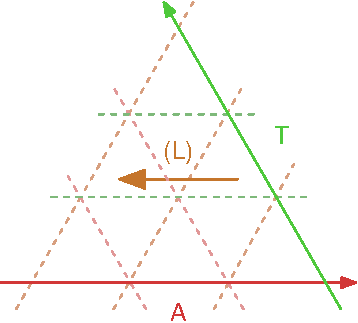
\includegraphics[height = 2cm]{Figures/JonasTable/TAl_iso-crop.pdf}  \\
  %%%% TLa
  $$\begin{aligned}
    &TL(A) \\
    &A = L - T
  \end{aligned}$$ &
  Helen lived to the age of 86 ($L$). When she had 20 years left ($T$) she must have been 66 ($A$). &
  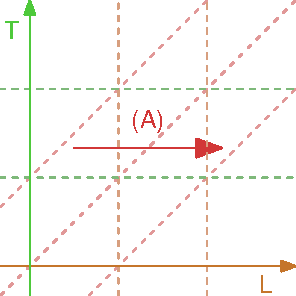
\includegraphics[height = 2cm]{Figures/JonasTable/TLa-crop.pdf} &
  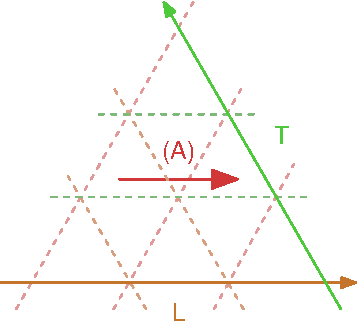
\includegraphics[height = 2cm]{Figures/JonasTable/TLa_iso-crop.pdf}  \\
  %%%% ALt
  $$\begin{aligned}
    &AL(T) \\
    &T = A - L
  \end{aligned}$$ &
  Tim is 34 years old ($A$) and will live to the age of 96 ($L$), leaving him 62 years ($T$) to settle affairs. &
  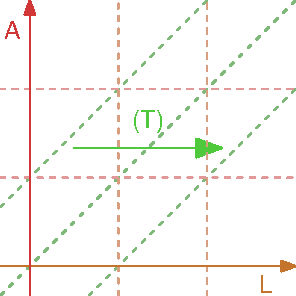
\includegraphics[height = 2cm]{Figures/JonasTable/ALt-crop.pdf} &
  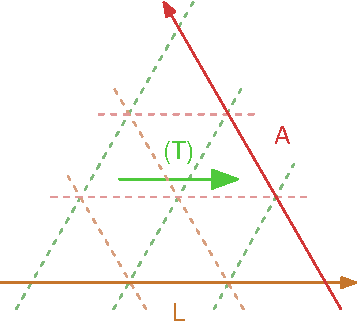
\includegraphics[height = 2cm]{Figures/JonasTable/ALt_iso-crop.pdf}  \\
  \midrule
  %%%%%%%%%%%%%%%%%%%%%%%%%%%%%%%%%%%%%%%%%%%%%%%%%%%%%%%%%%%%%%%%%%%%%%%%%%%%%
  \multicolumn{4}{c}{\textsc{Variants of LCD}} \\
  \midrule
  %%%% LCd
  $$\begin{aligned}
    &LC(D) \\
    &D = C + L
  \end{aligned}$$ &
  �ngels was born in 1940 ($C$) and she lived to be 64 ($L$), implying an
  untimely death in 2004 ($D$) &
  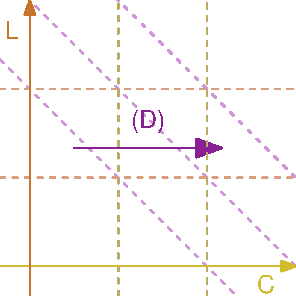
\includegraphics[height = 2cm]{Figures/JonasTable/LCd-crop.pdf} &
  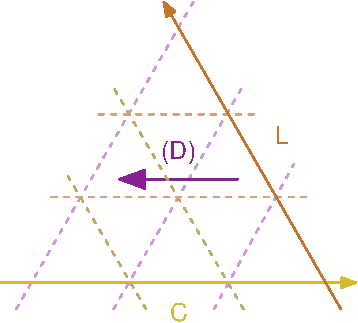
\includegraphics[height = 2cm]{Figures/JonasTable/LCd_iso-crop.pdf}  \\
  %%%% CDl
  $$\begin{aligned}
    &CD(L) \\
    &L = D - C
  \end{aligned}$$ &
  Pascal was born in 1893 ($C$) and died in 1964 ($D$), implying a lifespan of 71 ($L$), or so. &
  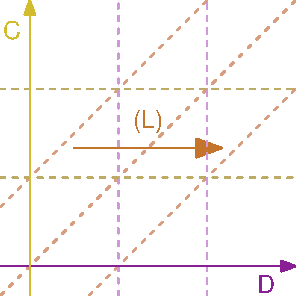
\includegraphics[height = 2cm]{Figures/JonasTable/CDl-crop.pdf} &
  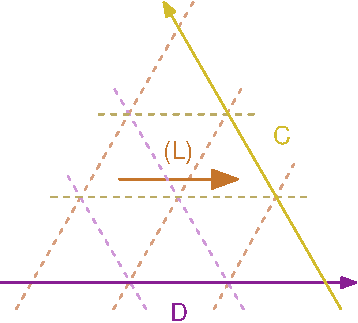
\includegraphics[height = 2cm]{Figures/JonasTable/CDl_iso-crop.pdf}  \\
  %%%% LDc
  $$\begin{aligned}
    &LD(C) \\
    &C = D - L
  \end{aligned}$$ &
  Margaret died in Dec., 1995 ($D$) with a completed lifespan of 96 ($L$), putting her birth year in 1900 ($C$). &
  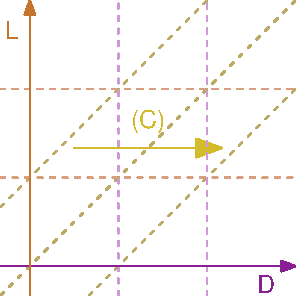
\includegraphics[height = 2cm]{Figures/JonasTable/LDc-crop.pdf} &
  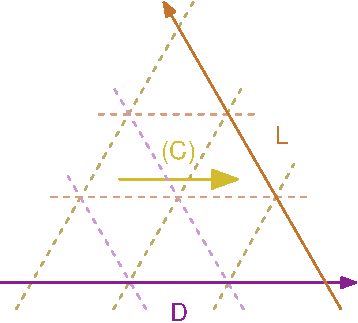
\includegraphics[height = 2cm]{Figures/JonasTable/LDc_iso-crop.pdf}  \\
  \midrule
  %%%%%%%%%%%%%%%%%%%%%%%%%%%%%%%%%%%%%%%%%%%%%%%%%%%%%%%%%%%%%%%%%%%%%%%%%%%%%
  \multicolumn{4}{c}{\textsc{The Uninformative Dyads}} \\
  \midrule
  %%%% LP
  $LP(-)$ &
  The $LP$ plane is \emph{non-informative}. No additional dimensions can be derived knowing just lifespan and period. &
  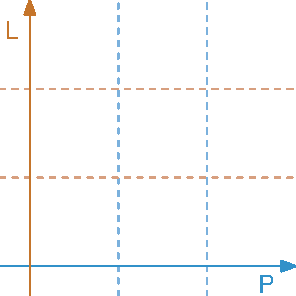
\includegraphics[height = 2cm]{Figures/JonasTable/LP-crop.pdf} &
   \\
  %%%% CT
  $CT(-)$ &
  The $CT$ plane is \emph{non-informative}. No additional dimensions can be derived knowing just cohort and thanatological age. &
  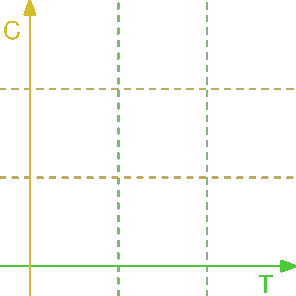
\includegraphics[height = 2cm]{Figures/JonasTable/CT-crop.pdf} &
   \\
  %%%% AD
  $AD(-)$ &
  The $AD$ plane is \emph{non-informative}. No additional dimensions can be derived knowing just death cohort and age. &
  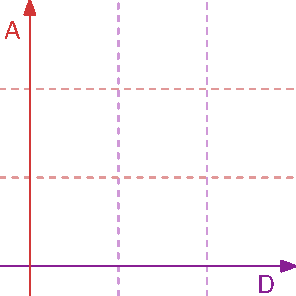
\includegraphics[height = 2cm]{Figures/JonasTable/AD-crop.pdf} &
    \\
  \bottomrule
\end{longtable}

Most of what we know about how rates change over age and time comes
from the very first juxtaposition in Table~\ref{tab:dyads}, $AP(C)$. While
$CP(A)$ and $AC(P)$ are statistically redundant, they are not fully redundant
in terms of geometric mappings if using Cartesian
coordinates, as demographers typically do. The other dyadic
juxtapositions can be considered as either rare or novel ways of structuring or
viewing temporal variation in demography.

There are $20=\binom{6}{3}$ ways to choose three time indices out of our
six, of which four form a triad identity: APC, TPD, TAL, and LCD.
Given the three time measures from any of the
triad identities, one can derive no further time measures. We therefore say
that the triad identities are themselves uninformative. If one selects three
random time indices that do not form any of these four triad identities
($20-4=16$ possibilities), this property does not hold. For instance, in the
triad $APT$, age and period are not sufficient to determine thanatological age.
Given the triad $APT$ one can however derive the remaining three time measures,
and for this reason we call it an informative triad.\footnote{We return to the
case of $APT$ and similar constructs in later sections.}

Visualizations of data structured by any dyad belonging to a triad identity
are inherently richer in information than are juxtapositions of uninformative
dyads. While there is no reason not to explore all possible
dyadic juxtapositions, triad identities have more apparent meaning, even in the absence of data, due to the underlying
relationship between measures. Each of the triad identities can accommodate some
version of a lifeline, for instance. In the following, we therefore lay
out the four primary diagrams that belong to the triad identities. 

\FloatBarrier
\subsection*{APC}%\tgh{APC}}
\FloatBarrier
The so-called Lexis diagram has long been used in demography as a conceptual
tool for structuring data, observations, and rate estimation, as inspiration for work
on statistical identification, and as the coordinate basis of contemporary
Lexis-surfaces \footnote{Some prefer the term Lexis \textit{surface}, while
others prefer to call them contour maps, heatmaps, or stereograms}.
Since the Lexis diagram could have been named for others
\citep{vandeschrick2001lexis,keiding2011age}, and since we compare with other
temporal configurations, let us refer to it as the APC diagram, as seen in
Figures~\ref{fig:APCrt} and~\ref{fig:APCeq}. 

\begin{figure} 
\caption{An APC diagram in two projections.}
\label{fig:APC}
\centering
\begin{subfigure}{1.1\textwidth}
\caption{Right angles}
\vspace{-5em}
\label{fig:APCrt}
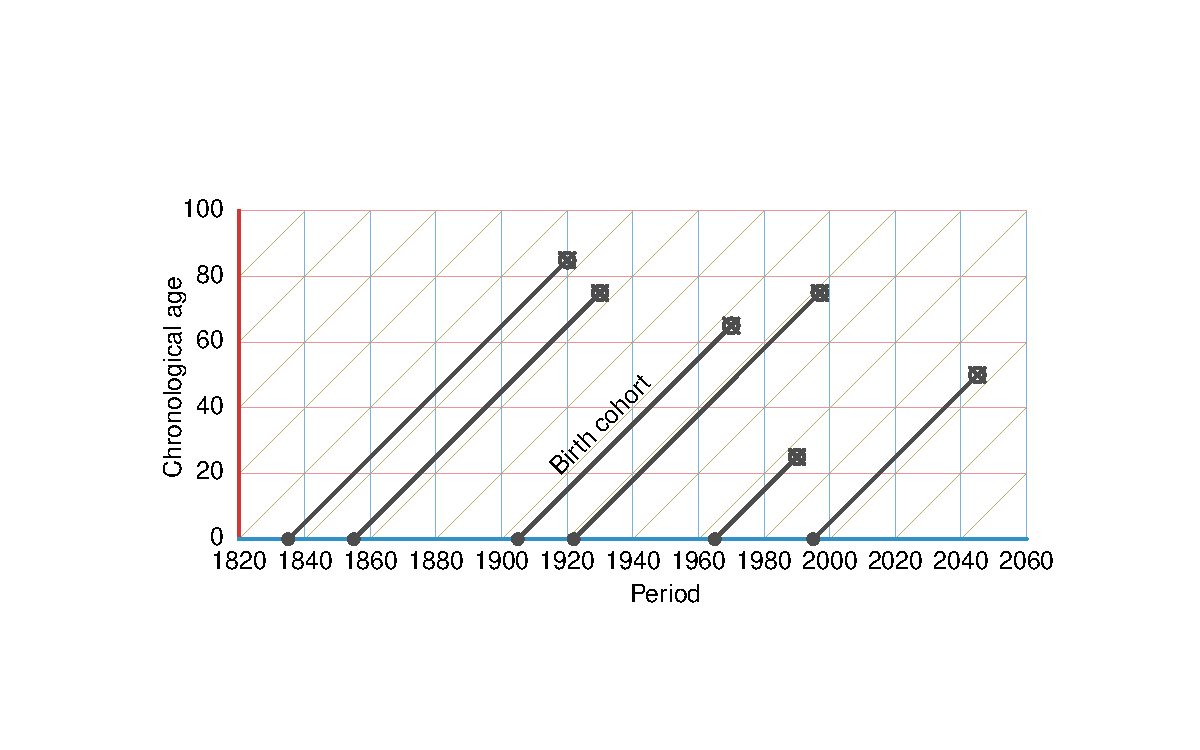
\includegraphics[scale=0.8]{Figures/APCrt.pdf}
\end{subfigure}
\\\vspace{-2em}
\begin{subfigure}{1.1\textwidth}
\caption{Isotropic}
\vspace{-6em}
\label{fig:APCeq}
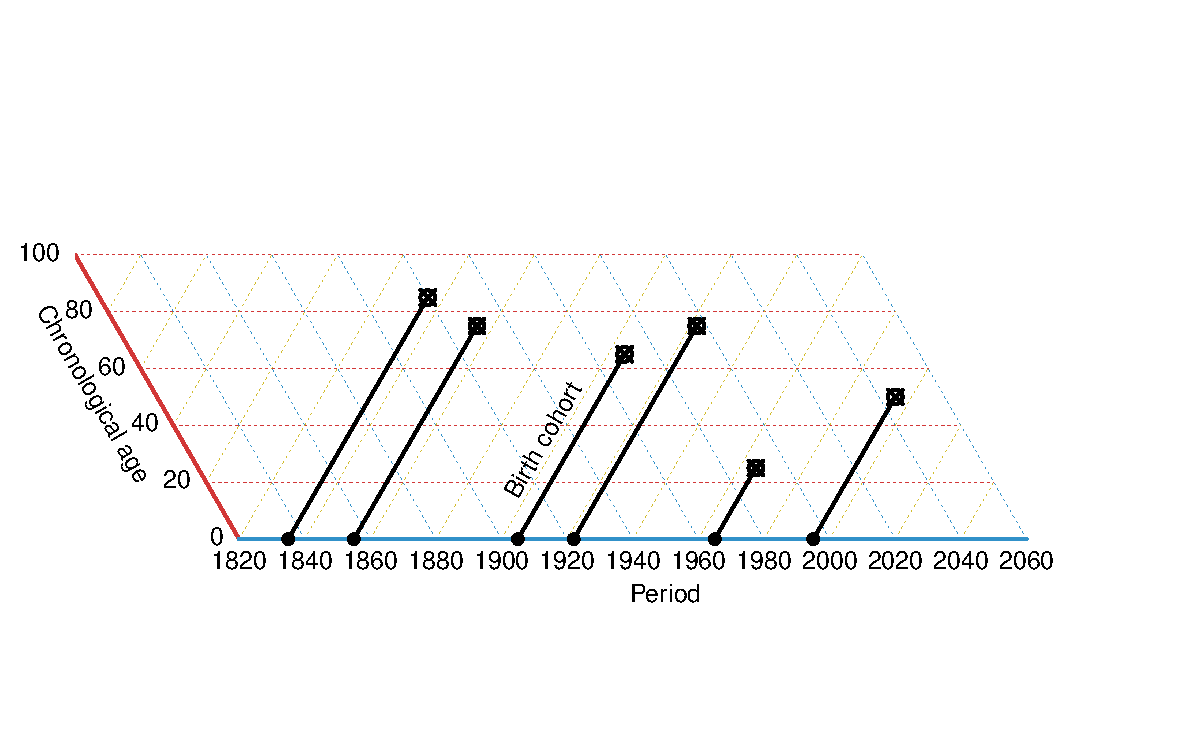
\includegraphics[scale=0.8]{Figures/APCeq.pdf}
\end{subfigure}
\end{figure}

The APC diagram in Figure~\ref{fig:APCrt} represents years lived on the y axis,
calendar years on the x axis, and birth cohorts as the right-ascending
diagonals. This is the most common of several possible configurations
of the APC dimensions. Individual lifelines (black) are aligned in the birth
cohort direction, starting with birth (filled circle) at chronological age zero, and death
(circled x). Any APC surface can be interpreted along each of these
three dimensions of temporal structure. 

\FloatBarrier
\subsection*{TPD}%\tgh{TPD}}
\FloatBarrier
Thanatological age (T), period (P) and death cohort (D) form a coordinate system
best imagined as the inverse of APC. One may take the same lifelines from
Figure~\ref{fig:APC} and realign them in descending fashion such that all
endpoints align to thanatological age 0, creating the diagram in
Figure~\ref{fig:TPD}.
Such diagrams have to our knowledge only appeared once in the literature, as a visual aid to a formal proof of the
symmetries between life lived and left in finite stationary populations \citep{pancho2015}. TPD coordinates may in general be used to arrange events or durations that are logically aligned (or may only be aligned) by time of
termination, and in general any
situation in which a terminal event aligns preceding patterns of variation.
Examples may include lifelines preceding deaths from infectious or acquired
conditions where the time of infection or acquisition is unknown. The main
justification for visualizing data in such coordinates is when birth cohort and
chronological age do not display regular empirical variation, but thanatological
age or death cohort do.

\begin{figure} 
\caption{A TPD diagram in two projections.}
\label{fig:TPD}
\centering
\begin{subfigure}{1.1\textwidth}
\caption{Right angles}
\vspace{-5em}
\label{fig:TPDrt}
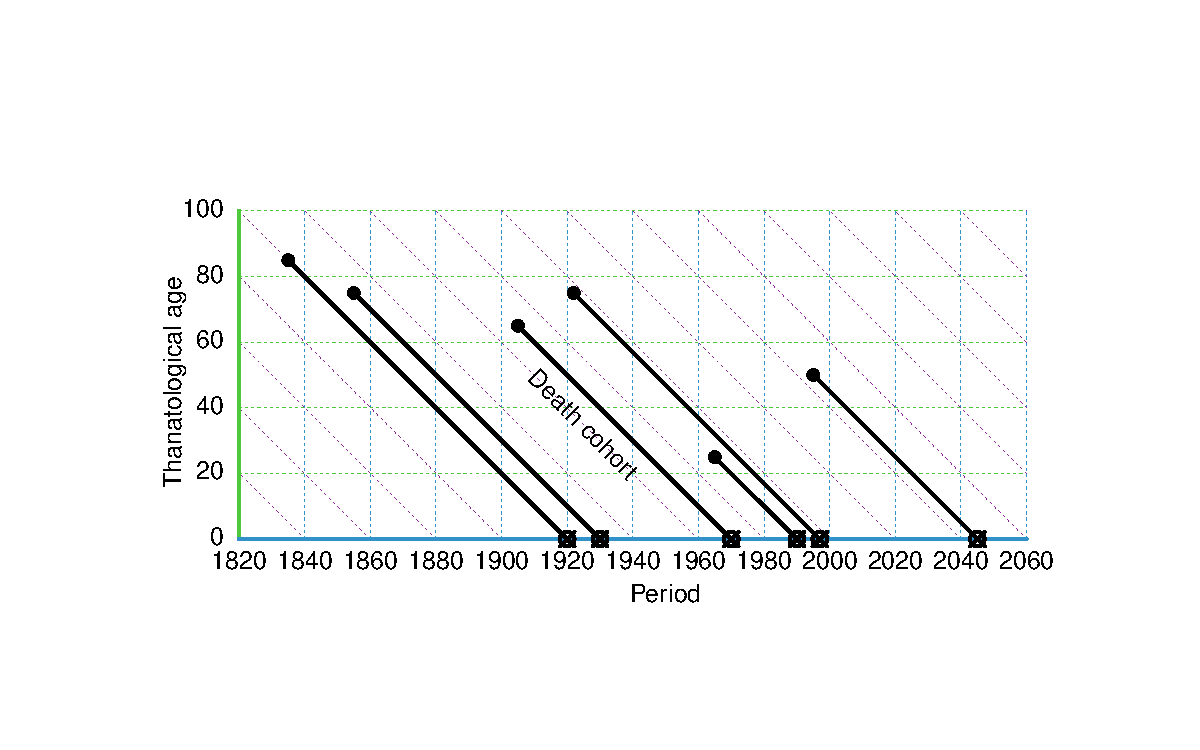
\includegraphics[scale=0.8]{Figures/TPDrt.pdf}
\end{subfigure}
\\\vspace{-2em}
\begin{subfigure}{1.1\textwidth}
\caption{Isotropic}
\vspace{-6em}
\label{fig:TPDeq}
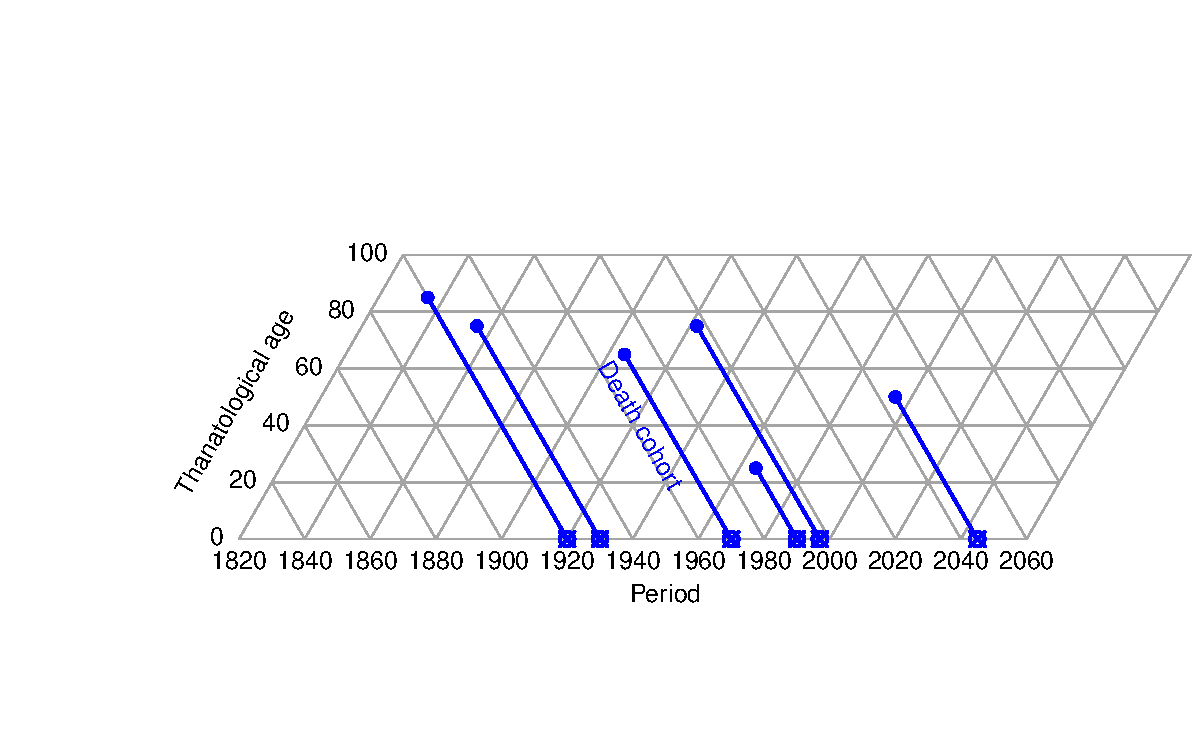
\includegraphics[scale=0.8]{Figures/TPDeq.pdf}
\end{subfigure}
\end{figure} 

\FloatBarrier
\subsection*{TAL}%\tgh{ATL}}
\FloatBarrier  
TAL is an appropriate coordinate
system to examine variation in processes over the lifecourse. Since
the lifecourse belongs to the cohort perspective, it is best to think of the TAL
plane as belonging to some particular birth cohort. Alternatively, an TAL
triangle may be taken as a cross-section along through the period dimension, a
sort of synthetic TAL plane. To our knowledge, the TAL diagram has only appeared
once in the literature, in an exploration and classification of late-life health
conditions \citep{riffe2015ttd}. The TAL diagram in Figure~\ref{fig:TAL}
contains no such indication of period or cohorts. The
lifelines depicted are identical those shown in APC Figure~\ref{fig:APC} and
TPD Figure~\ref{fig:TPD}.\footnote{The prior figures contained six lifelines
each, but since two of them were of equal length (75), they are overlapped in
Figure~\ref{fig:TAL} and appear to be five.} In this view, the user can
juxtapose some intensities that vary over the lifecourse with respect to years
lived and years left, and separated by lifespan, but time trends are blended
out, and cohorts overlapped.

\begin{figure}[h!] 
\caption{A TAL diagram in two projections.}
\label{fig:TAL}
\centering
\makebox[\textwidth][c]{
\begin{subfigure}{.48\textwidth}
\centering
\caption{Right angles}
\label{fig:TALrt}
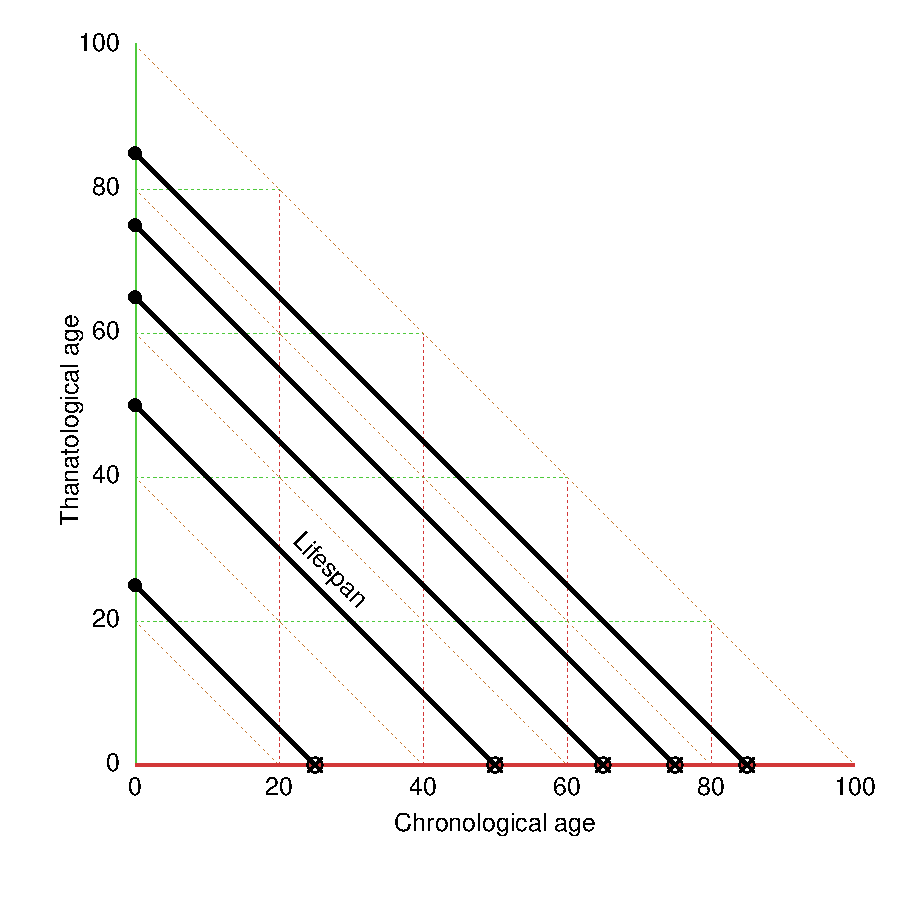
\includegraphics[scale=0.55]{Figures/TALrt.pdf}
\end{subfigure}
~~~~~
\begin{subfigure}{.48\textwidth}
\centering
\caption{Isotropic}
\label{fig:TALeq}
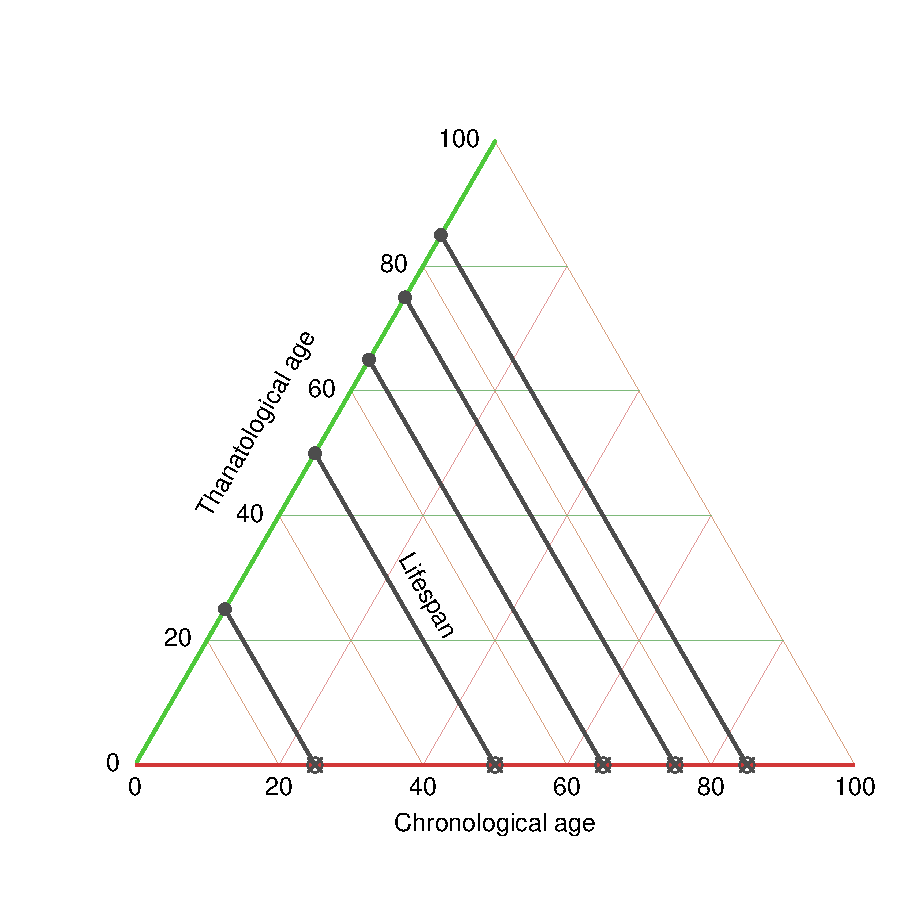
\includegraphics[scale=0.55]{Figures/TALeq.pdf}
\end{subfigure}
}
\end{figure} 

\FloatBarrier
\subsection*{LCD}%\tgh{CDL}}
\FloatBarrier

The LCD diagram completes our set of identities. It consists in an identity
between lifespans, birth cohorts, and death cohorts. This identity bears
resemblance to an APC surface of mortality, but we suggest some
differences due to blending out age. In figure~\ref{fig:LCDrt}, lifespans are
indexed by the y-axis, while birth cohorts are indexed by the x-axis. Lives are lived within birth
cohorts, engding with endpoint of blue lifelines in the figure. However, the
death cohort diagonals of the diagram are only valid for the endpoints of the
lifelines. To structure data on these three time measures implies ignoring
variation within the lifespan. 

\begin{figure} 
\caption{An LCD diagram in two projections.}
\label{fig:LCD}
\centering
\begin{subfigure}{1.1\textwidth}
\caption{Right angles}
\vspace{-5em}
\label{fig:LCDrt}
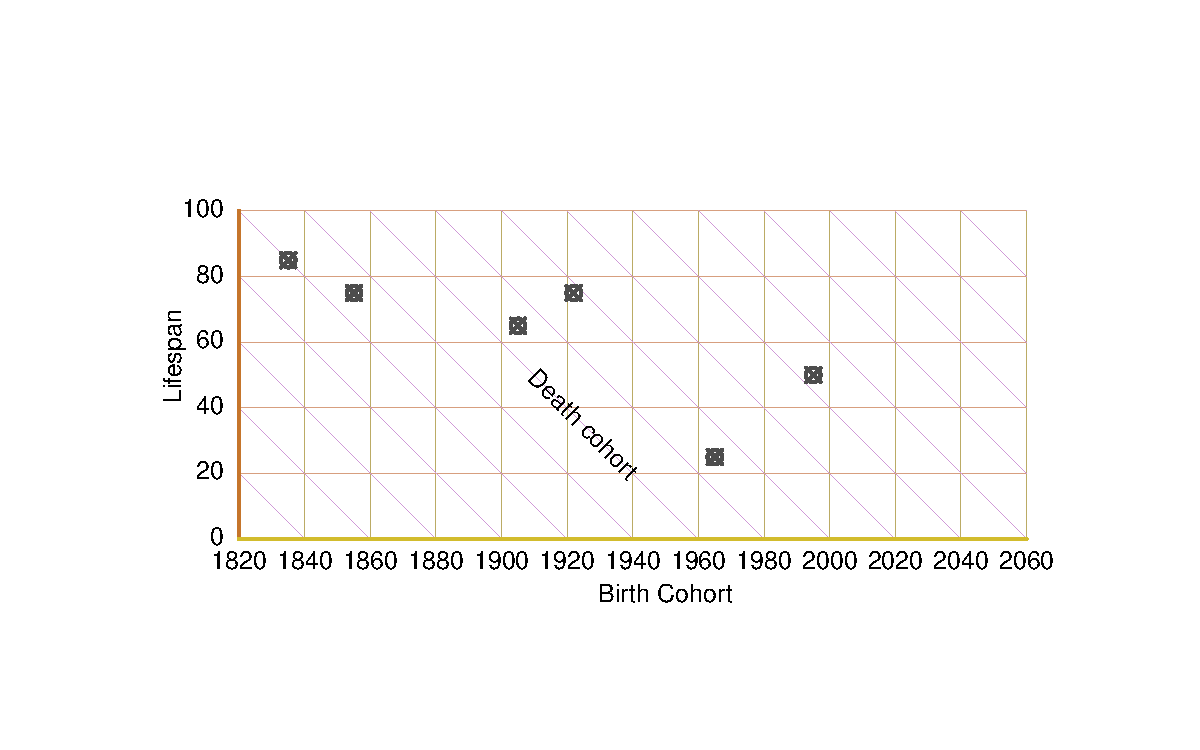
\includegraphics[scale=0.8]{Figures/LCDrt.pdf}
\end{subfigure}
\\\vspace{-2em}
\begin{subfigure}{1.1\textwidth}
\caption{Isotropic}
\vspace{-6em}
\label{fig:LCDeq}
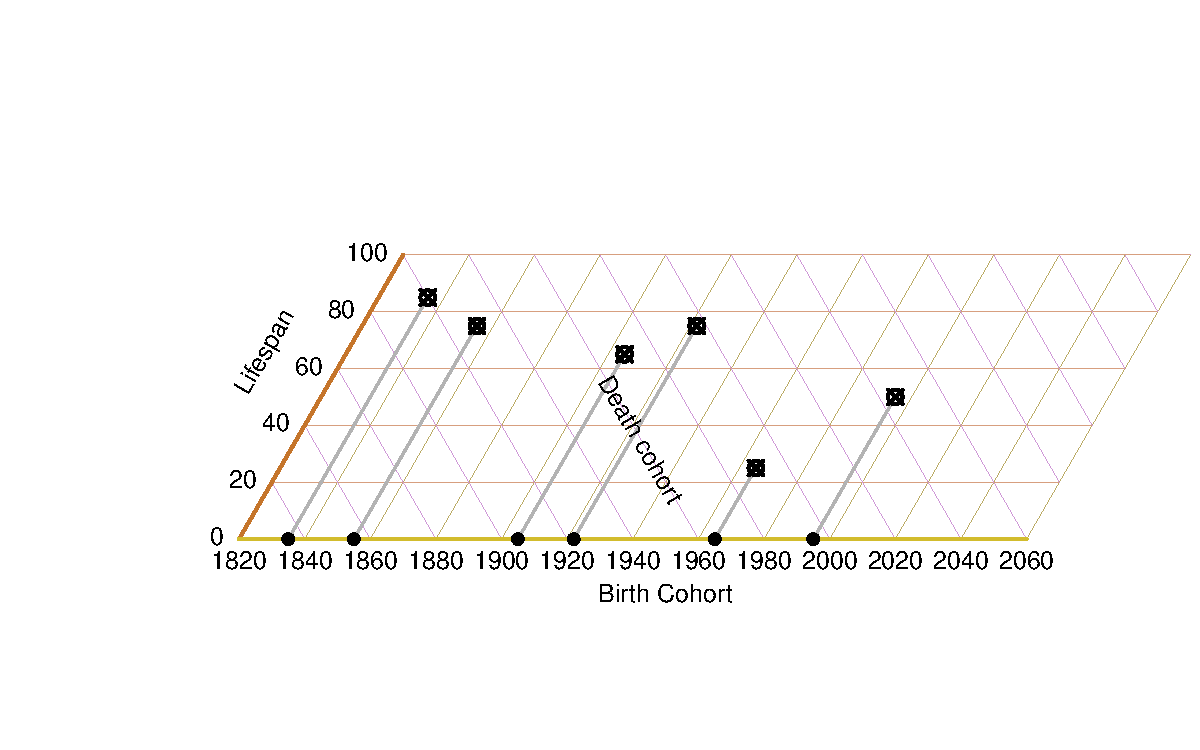
\includegraphics[scale=0.8]{Figures/LCDeq.pdf}
\end{subfigure}
\end{figure} 

We recommend this mapping for plotting surfaces of values that vary over time by
year of birth or death and that vary by lifespan, e.g., that are cumulative or
static over the lifecourse. Imagine an LCD surface of cumulative lifecourse
cunsumptive surplus or deficit, or anything else that might vary by lifespan and
over time, such as children ever born, or years of retirement. In a sense, APC
mortality surfaces already conform with this perspective, since the
intensities visualized mark the endpoints of lifelines. However a
mortality surface tells us only the relative intensity of death, which
translates to densities of life lines, but does not identify other kinds of
values.

Fertility surfaces are in this way very different from mortality surfaces, as they plot event intensities over the ages in which they occur. A health surface is more like a fertility surface than a mortality surface, but in this case proximity to death is an important time dimension. 

\FloatBarrier
\section*{A tetrahedron relates the six time indices.}
Each of the four above-mentioned triad identities may be thought of as a
two-dimensional plane fully defined by any two of its three constituent time
indices.
In this case, we may imagine any of the excluded time measures as capable of
providing depth, a potential $z-$coordinate, for the sake of a mental image.
Having a non-redundant third dimension implies a multitude of parallel planes
for the given triad identity, each plane belonging to a unique value of the
third time dimension. Any of the identities can be extended in this way to fill a space. A space derived by
extending any of the triad identies into its lacking dimension implies each of the
other triad identities, making a total of six time indices. In essence, the
four triad identities may be thought of as the four faces of a
tetrahedron. If an additional time measure is added to any face (triad
identity), the six demographic time indices can be derived, matching the six edges of the tetrahedron. This three-dimensional construct unifies the six indices of demographic time, and is the subject of this paper.

Let us first more rigorously define the previously-mentioned tetrahedron.
Luckily, the edges and vertices of a tetrahedron are easily rendered in a
two-dimensional graph, as seen in Figure~\ref{fig:tet}, with vertices labeled
in red and the six time indices labeled as blue edges. The reader may also imagine this graph as a transparent 3d object, in which case the four faces become apparent. There
are two intuitive ways to imagine the graph as 3d, either the vertex 4 is on top, and we gaze from a bird's-eye-view, or the vertex 4 is in the back, behind the other three vertices. Assume we
gaze from the top, for the sake of description.\footnote{The same graph
could be composed in four basic ways, depending on which triad-identity face
forms the base.
These are given in an appendix.} 

\begin{figure}[h!]
\centering
\caption{Graph of tetrahedron, with edges labeled by the six demographic time
indices.}
\label{fig:tet}
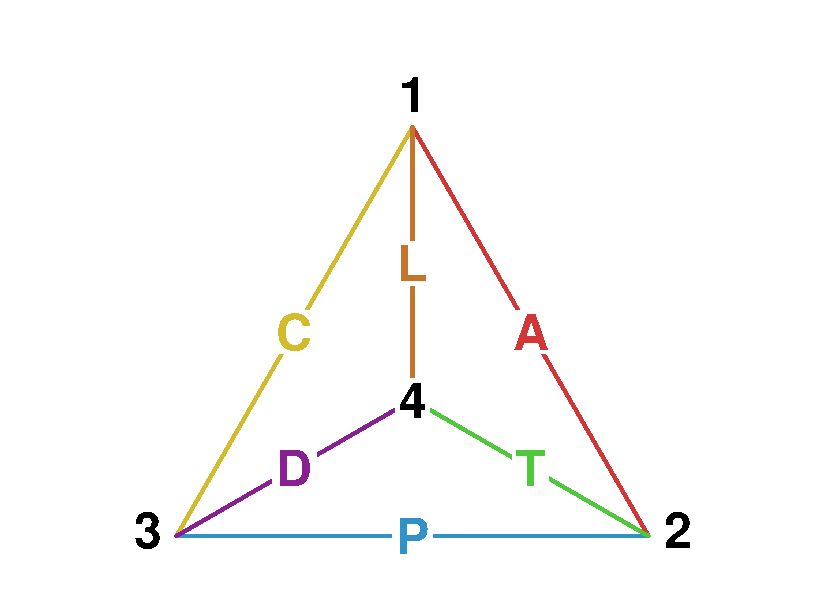
\includegraphics[scale=1]{Figures/TetraHedronVerticesEdges.pdf}
\end{figure}

\subsection*{Information criteria to derive the tetrahedron.}
The edges APC at the base define the much-studied APC plane. If the only
information we have is chronological age, period, and birth cohort (or just two
of these), then we have no access to the vertex 4. Each of the faces of the
tetrahedron has this quality. The South face TDP has no access to 1.
The Northeast face, ATL has no connection to 3, and the Northwest face
CDL lacks a connection to 2. The four triad identities that make up the faces of
the tetrahedron are stuck in ``flatland'' and do not yield the full 3d
space. However, the 16 other possible combinations of three time indices will recreate the full tetradhedron (hexad identity).


% PV: I suggest to replace the following paragraph, or at least to introduce
% this geometrical perspective somewhere in the text

%   TR: OK, I've commented it out. The removed paragraph sounds more like advice
%       on how to manually find all 20-16-12 triads without too much mental
%       labor. Maybe worth an appendix?
% TR: the vector description is probably more rigorous, so let's go with it.
%     We'll put some effort later into making it understandable for avg
%     demographers.

%\sout{For example, say we are at vertex \vt{1}, and we therefore have
%information on year of birth C, completed lifespan L, and
%chronological age A (see Figure~\ref{fig:tet4vert1}). Clearly, A and
%C imply P ($C+A=P$).
%A and L imply T ($L-A=T$). Finally, C and
%L imply D ($C+L=D$), and we have the full hexad
%identity. In the tetrahedron graph, we have three edges that connect to the
%four vertices. This is the essential property of a fully informed triad.
%It is easily verified that each vertex has this property.
%However, there are twelve other sets of three that also have this property. To
% locate these ``hidden'' triads, first note that each index has an
%opposite index, with which it shares no information. These pairs are
%A-D, L-P, and C-T, and can be found in Figure~\ref{fig:tet} as
%the three sets of perpendicular edges. Each of these pairs can be completed
% into a `fully-informed'' triad by the addition of any of the other four indices
%(thereby connecting the edges). Doing so for each of the opposite pairs will
%yield the remaining twelve triads.}

A geometrical analogy is pertinent at this point. Any pair of intersecting edges
of the tetrahedron may be interpreted as two vectors $\vec{u}$ and $\vec{v}$
that determine a 2-dimensional plane in a cartesian 3-dimensional
space ($\mathbb{R}^3$).\footnote{A 2d plane in a 3d space is determined by two linearly independent
vectors (with different direction) and a point, but the inclusion of a point is not
necessary for the intuitive analogy that we describe here.} Therefore, any third
vector $\vec{w}$ of that plane can be expressed as a linear combination of
$\vec{u}$ and $\vec{v}$ (formally, $\vec{w}=\alpha\vec{u}+\beta\vec{v}$ for some $\alpha, \beta \in \mathbb{R}$), which is usually
described by saying that $\vec{w}$ is linearly dependent on $\vec{u}$ and
$\vec{v}$.
A similar property can be derived from the information contained in the
tetrahedron: $A=P-C$ is a linear combination of $C$ and $P$ and it ``depends''
on them because they all belong to the same $APC$ plane. Analogously, $P=C+A$
``depends'' on $C$ and $A$, and $C=P-A$ ``depends'' on $P$ and $A$. Given that the faces of the tetrahedron represent the triad identities, any pair of intersecting edges has the same property: The third edge located in the same face of the tetrahedron can be determined by the first two by a simple linear relationship.

% code given in R/TetraCombos.R, lines 70-95
% PV: already created the new figure
%\begin{figure}[h!]
%\centering
%\caption{Graph of tetrahedron, edges belonging to the APC face highlighted.}
%\label{fig:tet4vert1}
%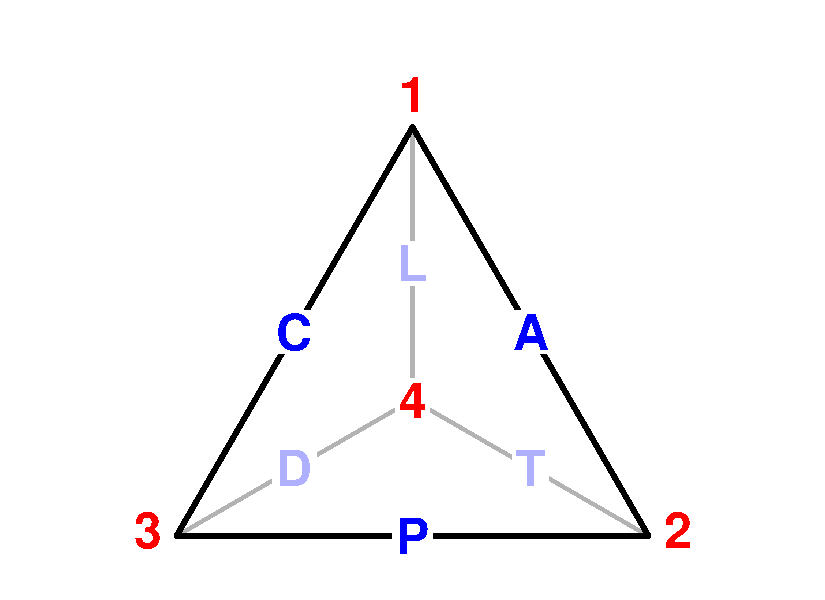
\includegraphics[scale=1]{Figures/tet4vert1New.pdf}
%\end{figure}
%\noindent 

Once a 2d-plane is defined in $\mathbb{R}^3$, an additional vector may be sufficient to cover a
3d-space. Nonetheless, this third vector needs to be linearly independent
of any pair of vectors of the 2d plane---that is, it cannot be expressed as a
linear combination of any two vectors on that plane. Again, an analogous
property can be observed in the tetrahedron: Say we only have information about the indices of the $APC$ plain; $A$, $C$ and $P$ are not sufficient to determine a thanatological age $T$, death cohort $D$, or lifespan $L$ (the three indices that do not belong to the $APC$ plane). So, $T$, $D$ and $L$ are ``independent'' of the overall information that can be extracted from the $APC$ plane. However, if two of the three constituent time indices of the $APC$ plane are known (the third one would be unnecessary as it could be derived from the other two), the additional information provided by any of the three ``independent'' indices $T$, $D$ or $L$ would be sufficient to cover the whole tetrahedron. For example, suppose we have information about thanatological age $T$ in addition to $C$ and $P$, then
$A=P-C$, $D=P+T$ and $L=T+A=T+P-C=D-C$. 

Hence, as with vectors in a 3d space, any
triad of indices that are independent of each other---that is, none of them can
be expressed as the sum or the difference of the other two---generates a full
hexad identity or, using an analogous terminology, covers the whole ``space'' of
demographic indices presented in this paper. Graphically, this is equivalent to
choosing any combination of three indices that do not belong to the same face
of the tetrahedron, i.e., that do not form one of the four triad identities
represented in Table~\ref{tab:triadids}.

\begin{table}[h]
\centering
\caption{The four triad identities on the tetrahedron (same orientation)}
\label{tab:triadids}
\begin{tabular}{cccc}
APC & TPD & ATL & CDL\\
\tg{APC} & \tg{TPD} & \tg{ATL} & \tg{CDL}
\end{tabular}
\end{table}

When graphed in this way, it is clearer that every triad identity surface lacks a connection to the opposite vertex of the tetrahedron. Table~\ref{tab:set3} gives the full set of 16 index-triads that are
complete in the sense that each of them implies the full hexad identity.

Note that the 12 possible pairs of intersecting edges on the tetrahedron are, in
fact, the informative dyads described in Table~\ref{tab:dyads}, whereas the uninformative dyads LP, CT, and AD are the pairs of opposite edges of the tetrahedron. As discussed, all 12 informative dyads generate one of the four triad identities in Table~\ref{tab:triadids}, but no dyad will generate the hexad
identity since a third ``independent'' time dimension is necessary.
Similarly, any quad of indices is sufficient to complete the hexad identity, as at least one of them will not belong to the same face of the tetrahedron, but a triad may be sufficient if they 
do not all belong to the same plane forming a triad identity.

\begin{table}[h]
\centering
\caption{All complete sets of three indices,
graphed given the previous orientation of the tetrahedron.}
\label{tab:set3}
\begin{tabular}{cccc}
ACD & ACL & ACT & ADL\\
\tg{ACD} & \tg{ACL} & \tg{ACT} & \tg{ADL}\\
ADP & ADT & ALP & APT\\
\tg{ADP} & \tg{ADT} & \tg{ALP} & \tg{APT}\\
CDP & CDT & CLP & CLT\\
\tg{CDP} & \tg{CDT} & \tg{CLP} & \tg{CLT}\\
CPT & DLP & DLT & LPT\\
\tg{CPT} & \tg{DLP} & \tg{DLT} & \tg{LPT}
\end{tabular}
\end{table}

\FloatBarrier
\subsection*{The extension of time axes.}
We have said that planes defined by the four triad identities are parallel to
the faces of the the above-described tetrahedron. In imagining this three-dimensional
relationship, we are no longer confined to the extent of the tetrahedron used thus far for orientation. Instead each of its edges extends a
certain distance in either direction.
It may therefore help to first consider the extension of each axis (or index).
Some indices have a lower bound of zero and an upper bound set by the maximum
length of life, $\omega$, while others are boundless. A, T, and L
are clearly in the range $[0,\omega]$.\footnote{It's best to imagine some number like 122.45 years, for $\omega$, rather than infinity. This is the longevity record at the time of this writing. Jeanne L. Calment would have had
$T=122.45$ at birth, $A = 122.45$ at death, and $L=122.45$ for
her entire life.} P, C, and D are bounded only by the inception and extinction of
our species, but may be thought of as boundless for practicality, or benchmarked
to our earliest and most recent observations for even more
practicality.\footnote{We explain the choice of the word ``benchmarked''. Say
we have a data series that runs from 1751 to 2011, and an upper age
interval of $110+$. Then we could say that P is in the range $[1751,2011]$,
but by another reading, P must range from at least as early as the earliest
C and until at least as late as the latest D. Someone dying at 110 in 1751
had a C of 1640, and an infant born in 2011 that is destined to live to 110
will die in 2121. In this case a P that \textit{contains} the observed
population will extend well before and after the observed data series, even
moreso if we take into account that $\omega > 110$.} As an abstraction,
however, the dimension of calendar time in this model is infinite. Of the four
triad identities, only one lacks an unbounded dimension, the TAL. Adding
the absent dimension to TAL therefore makes its 3d extension boundless. In
this way, we may imagine a prism-like construct, where T, A, and L, compose
the faces of a triangular cross-section of the prism, which extends infinitely
``through'' the triangle.
We can think of the TAL triangle passing through time, extending the population
forward to infinity. In this case, the TAL triangle may take either the period
or cohort perspective, and this will be explained later. 

There are also
numerous ways that this three dimensional construct can be proportioned, of
which we present two in this paper. The first stems from the respect given to
right angles in the most common representation of the Lexis diagram. For this reason, it will likely be
the most intuitive rendition of the model, and it will be presented first. The
second version presented is isotropic with respect to time units in each of the
six temporal indices. In this case, the four tripartite identities are based on
equilateral triangles between their three constituent indices, and the four
planes are joined together such that each is parallel to a face from the regular
tetrahedron, a construct known in geometry as an octahedral-tetrahedral
honeycomb.

\section*{Intersecting planes}

The APC, TPD, TAL, and CDL planes can be conceived of either as
\textit{compressions} of this 3d space, or as cross-sections of the 3d space. To
compress space in this sense is to ignore the missing dimension,
whereas a cross-section sets a given triad identity against a particular
position of the absent dimension. This is a more general sense of the term
\textit{cross-section} than is often used in the demographic literature, where
it typically implies a period cross-section.
APC has thus far always been treated as a compression in this sense.
A compressed TPD diagram has thus far only appeared in \citet{pancho2015} as an aid in proving the symmetries between chronological and thanatological age in stationary populations, and a cross-sectional one has
never appeared.
Cross-sectional TAL diagrams and surfaces have thus far only appeared in
\citet{riffe2015ttd}. This TAL usage was selected for the 1915-1919 birth cohort, and therefore belongs to the 3d space,
\raisebox{-.25\height}{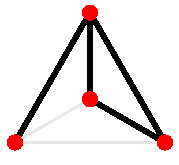
\includegraphics[scale=.15]{Figures/triadtable/ATLC.pdf}}.
We have been unable to locate an example in the literature of a compressed
TAL diagram, but it seems plausible one will have arisen in the field of
biology, albeit with no relation to the present discourse. We suppose
that LCD diagrams of any kind are yet-unknown.

A simultaneous juxtaposition of the six demographic time measures has also never
appeared in the literature, either as a visual diagnostic or in any line of
inquiry or argumentation, although there are some novel temporal
juxtapositions in the literature on event analysis of
big data \citep[see e.g.,][]{watson2015timemaps}.

 \section*{APCTDL}
There are various ways in
which one might visualize the 3d space of demographic time, emphasizing
different planes or intersections. In figure~\ref{fig:apctTAL} we offer a view
of the hexad identity, where birth-cohort TAL cross-section planes are placed in
sequence. The most recent TAL plane, for year $t$, is placed in the front,
whereas past TAL planes are stacked behind it in century intervals. In this
view, the emphasis is on how the juxtaposition of thanatological age, chronological age, and lifespan change over time. This is the view used in \citet{riffe2015ttd}, albeit for a single birth cohort only.
The base of this figure is the APC plane. Each of the TAL planes therefore sits
atop a single birth cohort line from the APC plane that makes up the base of the
figure. 

A property of the model that we propose is isotropy, i.e,
the time units with respect to each time measure are proportional.
In geometry nomenclature, the isotropic 3d space that results from this model is
called the tetrahedral-octahedral honeycomb, a kind of space-filling
tessellation. Constructs following this geometry exist in nature, in other
theoretical settings, and in man-made structures. 


\begin{figure}[!h]
\centering
\begin{adjustwidth}{-2em}{-2em}
\caption[cap]{Birth cohort TAL planes over time}
\label{fig:apctTAL}
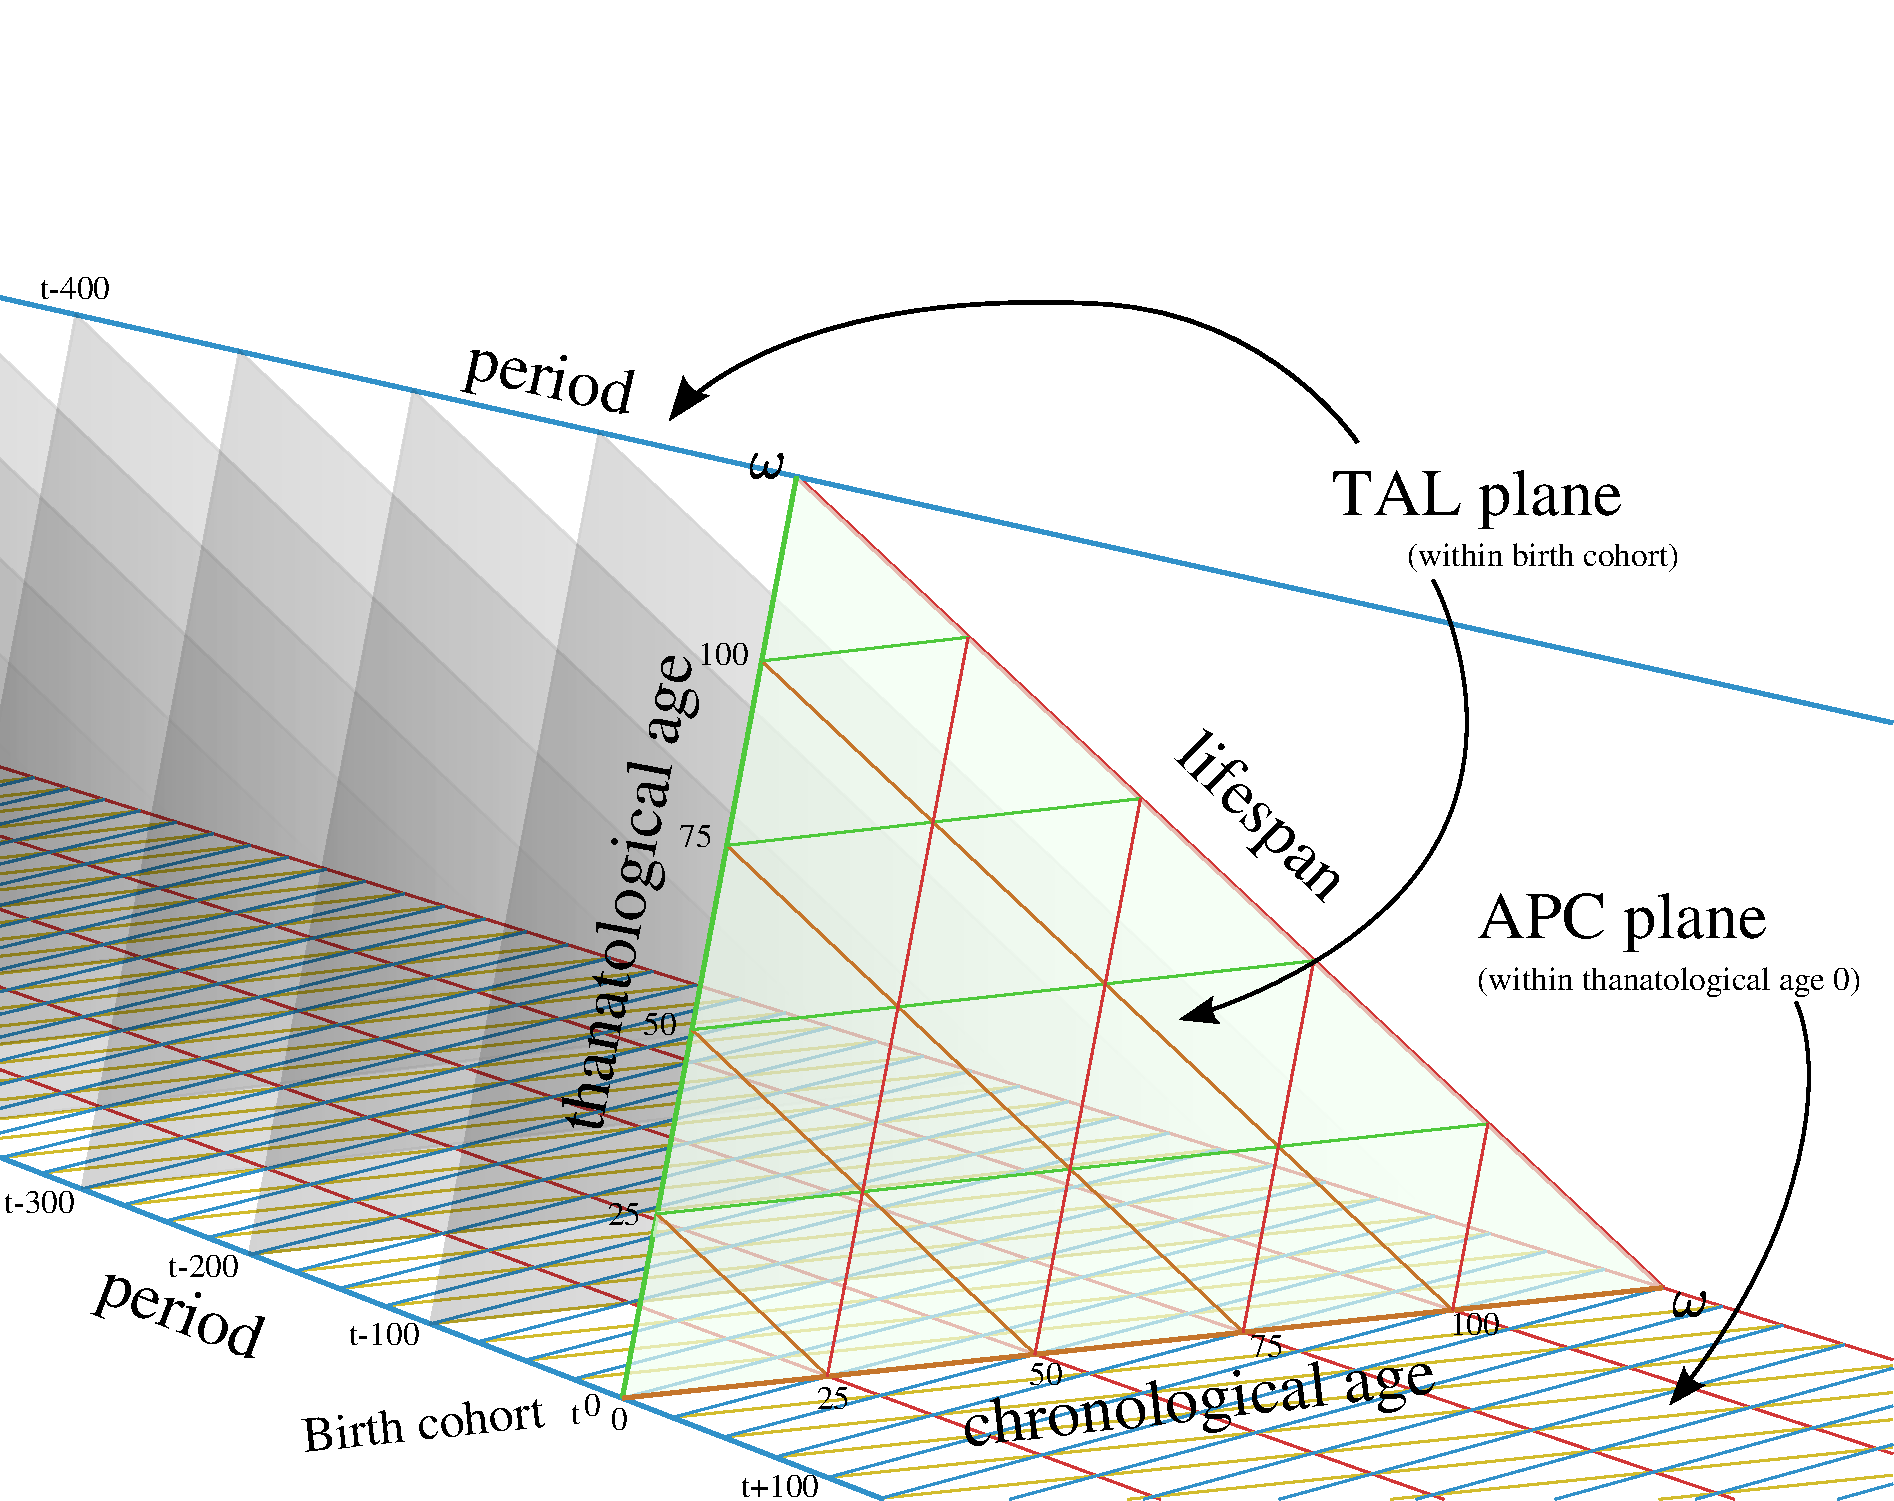
\includegraphics[scale=.5]{Figures/TALisomarkedup.pdf}
\end{adjustwidth}
\end{figure}



%In Lexis-nomenclature, the 3d projections of an AP square, and AC or PC
%parallelograms are all congruent shapes known as regular trigonal trapezohedra
%(RTT). The orientation
%of a given RTT uniquely defines the Lexis shape in question. Similar constructs
%exist in the other time dimensions. 

%This three
%dimensional space is not only useful for the sake of formalizing observed
% temporal relationships, but also for enclosing demographic time in the past and future (e.g., before the first census and after the most recent census).

\section*{Discussion}
The contemporary practice of demography is based on the premise that vital
rates, and other kinds of rates over the lifecourse, are the truest measure of
demographic quantum. Rates are paramount because they tend to vary in
empirically regular ways. The scalings and movements of primary vital rates fall
within a limited range for humans. For this reason, many of the methods of
demography are developed to estimate rates, independent of population composition, or to
partition crude magnitudes into the effects of population age structure and
pure vital rates. Controlling for age is in a more general sense controlling for
temporal variation in stocks. 

The best way to seek regular patterns in variation
is via data visualization. The coordinate system proposed in this paper is
conceived as one adequate to capture all such variation, and we suggest its use
for visualizing data, probably via small multiples of successive time slices
parallel to any of the four triad identities. Such strategies at this time are
exploratory and speculative, but much may be learned from how quantities that
vary through 3d volumes are visualized in other disciplines, such as
neuroscience or geology.

The techniques used to age-standardize mortality and fertility estimation are at
times applied to other kinds of transitions over the life course. For example,
one may estimate an age pattern to some degenerative disease, or the
ability to carry out some common activities of daily life. Much of the
regular temporal variation for such conditions is by thanatological age or
lifespan, rather than chronological age. Apparent chronological age patterns for
such conditions are artifactual and do not represent the same kind of
intrinsic meaning as does the age pattern of mortality. Further kinds of
temporal standardization must be developed in order to measure and understand
the natural patterns of such conditions over the lifecourse. The measurement of such conditions may benefit from consideration of the complete model presented in
this paper. To this end, Table~\ref{tab:set3} provides all combinations of
information that are sufficient to derive the full space. Some panel surveys
with mortality followups already provide the requisite information, as do
linkable registers that include items such as health measures or proxies and
relevant dates of birth, observation, and death.

Mortality determines three of the dimensions of
demographic time, and it therefore makes little sense to model mortality using
all six time measures. Any of the six measures may be pertinent in the case of
conditions and states that vary over and within the lifecourse. Fertility is one
such within-lifecourse event, although it may still turn out that most important
variation in fertility is captured by APC. This remains to be seen until
adequate data is brought to bear on the question. The most obvious application
for the present model, given data commonly (and publicly) available at this
time, are late-life health conditions, although there may be other substantive
areas of application that have not occurred to us.



\FloatBarrier

%\begin{appendices}
%\section{Variants of tetrahedron graph}
%The graph depicted in Figure~\ref{fig:tet} could be drawn with any of the
%four vertices in the middle of the triangle (as well as other inversions
%and rotations).
%These would all serve equally well to present the same aspects of the model,
% and we have no insight as to whether one of these renditions is more or less
%intuitive. Figure~\ref{fig:app:tet} provides four perspectives on the
%tetrahedron, for the case that this aids in understanding. The reader may make
% a paper tetrahedron, with labeled edges and vertices to be convinced that
%these are identical graphs.
%\begin{figure*}
%        \centering
%        \caption{Some variants of the graph of the APCTDL tetrahedron.} 
%         \label{fig:app:tet}
%        \begin{subfigure}[b]{0.475\textwidth}
%            \centering
%            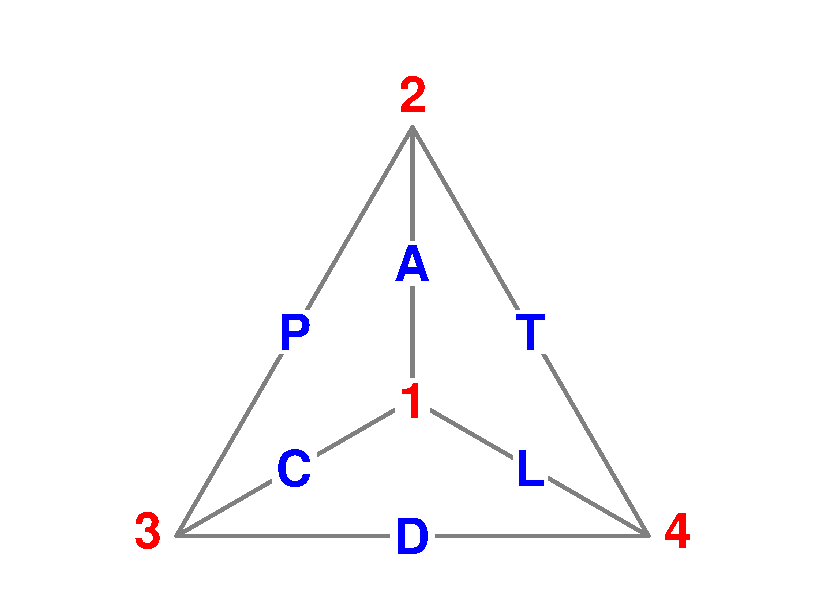
\includegraphics[width=\textwidth]{Figures/Tetra1.pdf}
%           \caption{\small Vertex \vt{1} in middle. APC Northwest.}
%            \label{fig:tet1}
%        \end{subfigure}
%    \hfill
%        \begin{subfigure}[b]{0.475\textwidth}  
%            \centering 
%            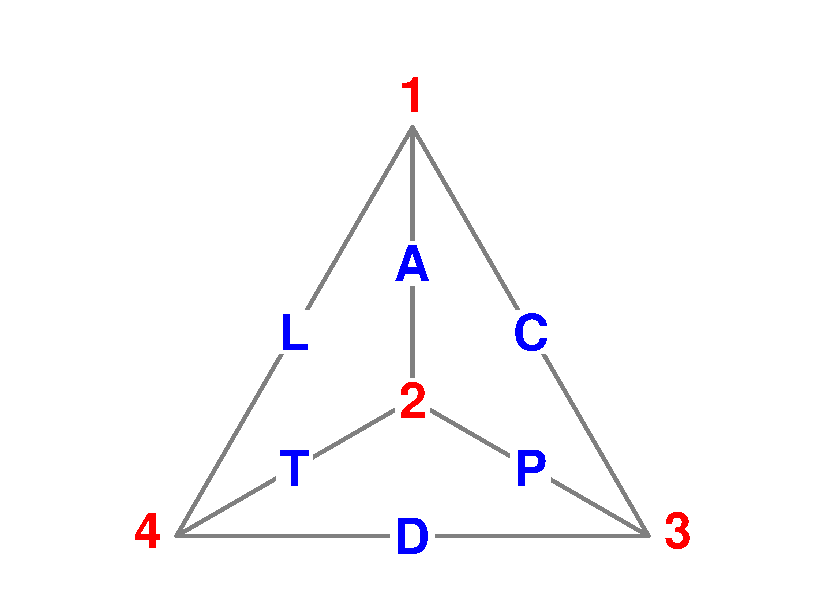
\includegraphics[width=\textwidth]{Figures/Tetra2.pdf}
%           \caption{\small Vertex \vt{2} in middle. APC Northeast.}
%            \label{fig:tet2}
%        \end{subfigure}
%        \vskip\baselineskip
%        \begin{subfigure}[b]{0.475\textwidth}   
%            \centering 
%            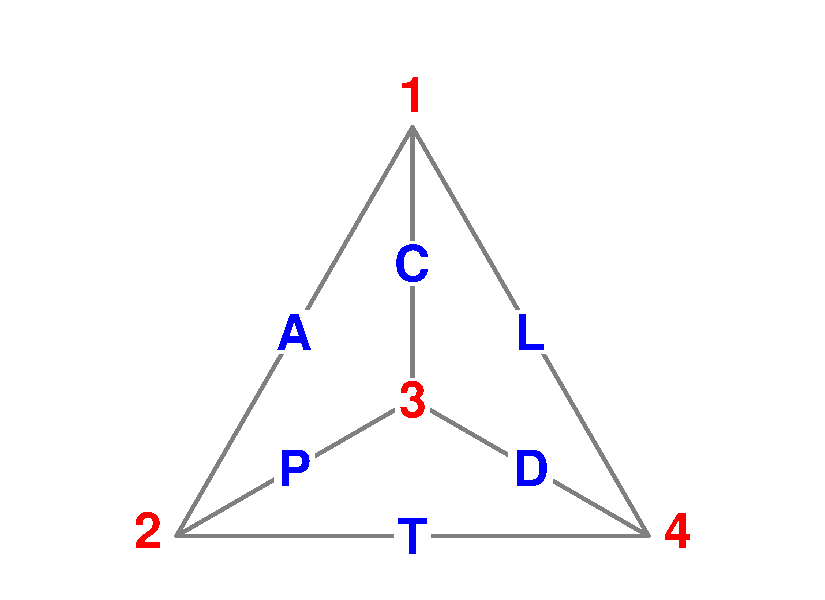
\includegraphics[width=\textwidth]{Figures/Tetra3.pdf}
%           \caption{\small Vertex \vt{3} in middle. APC Northwest.}
%            \label{fig:tet3}
%        \end{subfigure}
%        \quad
%        \begin{subfigure}[b]{0.475\textwidth}   
%            \centering 
%            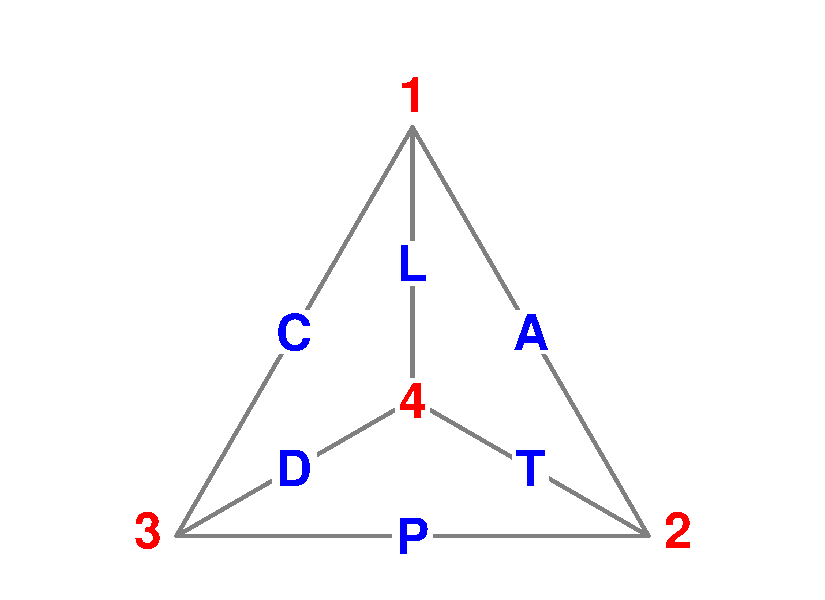
\includegraphics[width=\textwidth]{Figures/Tetra4.pdf}
%            \caption{\small Vertex \vt{4} in middle, as in
%            Figure~\ref{fig:tet}. APC base.}
%            \label{fig:tet4}
%        \end{subfigure}
%    \end{figure*}
%\end{appendices}
%\FloatBarrier

\bibliographystyle{plainnat}
  \bibliography{references} 



\end{document}